\documentclass[conference]{IEEEtran}
\IEEEoverridecommandlockouts

\usepackage{cite}
\usepackage{amsmath,amssymb,amsfonts}
\usepackage{algorithmic}
\usepackage{graphicx}
\usepackage{textcomp}
\usepackage{xcolor}
\usepackage{forest}

\def\BibTeX{{\rm B\kern-.05em{\sc i\kern-.025em b}\kern-.08em
    T\kern-.1667em\lower.7ex\hbox{E}\kern-.125em}}

\begin{document}

\title{A Comparative Study of Positional Encoding Methods for Length Extrapolation}

\author{
\IEEEauthorblockN{Prasiddha Raj Poudel}
\IEEEauthorblockA{
Department of Electronics and Computer Engineering\\
Thapathali Campus, Tribhuvan University\\
Kathmandu, Nepal\\
prasiddha.080bct027@tcioe.edu.np
}
}

\maketitle

\begin{abstract}
Transformer models rely on self-attention to process input sequences. Self-attention does not preserve token order, so positional encoding supplies sequence information during training and inference. The choice of positional encoding determines how well a model generalizes to sequence lengths beyond its training window. This paper presents a comparative empirical study of three positional encoding paradigms: Learned Absolute Positional Embedding, Rotary Positional Encoding (RoPE), and Attention with Linear Biases (ALiBi). We evaluate three pre-trained models (GPT-2, Pythia-160M, BLOOM-560M) under zero-shot inference on a free-tier Google Colab T4 GPU at sequence lengths from 512 to 8,192 tokens, measuring perplexity, needle-in-a-haystack retrieval accuracy, and per-token latency. Results show that all methods retrieve effectively within their training windows, but neither RoPE nor ALiBi enables reliable zero-shot extrapolation beyond them: RoPE perplexity degrades $48\times$ at $2\times$ training length and retrieval collapses to 0\%, while ALiBi retains perfect retrieval only through its training window. These findings corroborate that post-training scaling methods remain necessary for meaningful length extrapolation.
\end{abstract}

\begin{IEEEkeywords}
Transformer, Positional Encoding, Length Extrapolation, Self-Attention, RoPE, ALiBi
\end{IEEEkeywords}

\section{Introduction}
\label{sec:introduction}

Transformer architectures have become the standard foundation for natural language processing \cite{vaswani2017,touvron2023}. Their primary strength lies in self-attention, which models dependencies across sequence tokens. However, self-attention alone is permutation-invariant. A transformer treats input tokens as an unordered set unless explicit positional information is provided \cite{vaswani2017}.

Positional encodings solve this by assigning position representations to tokens. Early models used absolute encodings, such as fixed sinusoidal functions or learned position embeddings \cite{vaswani2017,devlin2019,radford2019}. While effective within the training window, absolute encodings degrade rapidly when evaluating sequences longer than those seen during training \cite{press2022}.

To solve this length extrapolation problem, recent architectures use relative rotations or attention score biases. Rotary Positional Encoding (RoPE) rotates query and key vectors in complex space \cite{su2024roformer}, while Attention with Linear Biases (ALiBi) adds distance-based penalties directly to attention logits \cite{press2022}.

This paper presents a comparative empirical study evaluating Learned Absolute embeddings, RoPE, and ALiBi. Because training large models from scratch requires prohibitive computing resources, we design a resource-constrained zero-shot evaluation methodology and test open-weight models (GPT-2, Pythia-160M, BLOOM-560M) on Google Colab free-tier hardware.

The contributions of this paper are:
\begin{itemize}
\item A structured review of absolute, rotary, and bias-based positional encoding paradigms.
\item A practical, resource-constrained evaluation methodology for testing length extrapolation, retrieval depth, and inference efficiency.
\item Empirical results on perplexity, needle retrieval, and latency for GPT-2, Pythia-160M, and BLOOM-560M at context lengths from 512 to 8,192 tokens.
\end{itemize}

\section{Literature Review}
\label{sec:literature}

Research on positional encoding has progressed from absolute representations to methods designed specifically for long-context inference. Rather than describing each method in isolation, this section compares methods along four practical axes: zero-shot extrapolation capability, recency and retrieval trade-offs, fine-tuning requirements, and computational cost. Figure~\ref{fig:taxonomy} summarizes the taxonomy, following the structure proposed in a recent survey \cite{zhao2024survey}.

\begin{figure*}[htbp]
\centering
\footnotesize
\begin{forest}
for tree={
  parent anchor=south,
  child anchor=north,
  align=center,
  edge={-latex},
  s sep+=6pt,
  l sep+=14pt,
  inner sep=2pt,
  edge path={
    \noexpand\path[\forestoption{edge}]
      (!u.parent anchor) -- +(0,-4pt) -| (.child anchor)\forestoption{edge label};
  },
}
[Positional Encoding
  [Absolute
    [Sinusoidal]
    [Learned]
  ]
  [Relative
    [Shaw]
    [T5]
  ]
  [Rotary
    [RoPE]
    [Position\\Interpolation]
    [YaRN]
    [Frequency\\Scaling]
  ]
  [Bias-based
    [ALiBi]
    [KERPLE]
  ]
  [Implicit /\\Augmented
    [NoPE]
    [Randomized\\PE]
  ]
]
\end{forest}
\caption{A taxonomy of positional encoding methods for Transformer models.}
\label{fig:taxonomy}
\end{figure*}

\subsection{Zero-Shot Extrapolation and Fine-Tuning}

Learned absolute embeddings cannot extrapolate at all: positions beyond the training range have no corresponding embedding \cite{devlin2019,radford2019,press2022}. Sinusoidal encoding is defined analytically for any position, but models rarely learn the underlying structure well enough to generalize \cite{vaswani2017,press2022}.

Relative encodings extrapolate better because they depend on token distance. RoPE extrapolates moderately well out of the box, though high-frequency dimensions oscillate unpredictably at long distances \cite{su2024roformer,sun2022lex}. ALiBi and KERPLE achieve the strongest zero-shot extrapolation, since their bias term is well-defined at any length with no learned positions \cite{press2022,chi2022}. BiPE improves length generalization by separating intra-segment absolute from inter-segment relative encoding \cite{he2024bipe}. Notably, NoPE occasionally outperforms ALiBi and RoPE on length generalization, suggesting that stable attention behavior is more fundamental than the specific encoding mechanism \cite{kazemnejad2023}.

Regarding fine-tuning: absolute embeddings cannot be extended without retraining \cite{press2022}. ALiBi and KERPLE require no fine-tuning since their bias function has no learned parameters \cite{press2022,chi2022}. Position Interpolation compresses coordinates and needs brief fine-tuning \cite{chen2023}. YaRN achieves comparable results with fewer fine-tuning steps \cite{peng2023yarn}.

\subsection{Recency Bias and Retrieval}

ALiBi and KERPLE penalize distance explicitly, producing strong recency bias that hinders long-range retrieval \cite{press2022,chi2022}. RoPE does not impose a hard distance penalty but has milder, less predictable recency bias from phase-shifting instability at long ranges \cite{su2024roformer,sun2022lex}. CABLE's content-conditioned bias adjusts per token, potentially softening recency effects while preserving extrapolation \cite{veisi2025cable}.

\subsection{Computational Cost}

RoPE rotates query and key vectors with element-wise multiplication, adding negligible latency and zero extra parameters \cite{su2024roformer}. ALiBi is even cheaper, applying a static bias addition to attention scores \cite{press2022}. Learned embeddings add parameters proportional to the context limit but have negligible runtime overhead. CABLE's per-head network is more expensive than ALiBi's fixed slope but still far cheaper than a full attention layer \cite{veisi2025cable}. Position Interpolation, YaRN, and frequency rescaling preserve the computational profile of the base RoPE model \cite{chen2023,peng2023yarn,liu2024scaling}.

\section{Methodology}
\label{sec:methodology}

\subsection{Theoretical Framework and Justification}

Self-attention compares query and key vectors using similarity scores. Without explicit positional encoding, self-attention treats inputs as unordered sets \cite{vaswani2017}. Positional encodings break this symmetry by injecting position information into the attention computation. The design of a positional encoding determines how well the attention mechanism generalizes when input length exceeds the training context window.

We evaluate three core paradigms representing modern language model architectures:
\begin{enumerate}
\item \textbf{Learned Absolute}: Embedding vectors added to input tokens (e.g., GPT-2).
\item \textbf{Rotary (RoPE)}: Complex rotations applied directly to query and key vectors \cite{su2024roformer} (e.g., Pythia, Qwen).
\item \textbf{Linear Biases (ALiBi)}: Distance penalties added directly to attention logits \cite{press2022} (e.g., BLOOM).
\end{enumerate}
Comparing these three paradigms isolates how position mechanics affect context length extrapolation.

\subsection{Research Design}

We use an empirical zero-shot evaluation design. Training large transformer models from scratch requires extensive GPU hardware beyond typical computing constraints. Instead, we evaluate pre-trained open-weight models representing each paradigm on a single Google Colab free-tier T4 GPU.

We execute forward-pass evaluations across sequence lengths $L \in \{512, 1024, 2048, 4096, 8192\}$ across three tasks:
\begin{enumerate}
\item \textbf{Perplexity Extrapolation}: Measure language modeling perplexity on long-form text as sequence length scales.
\item \textbf{Needle-in-a-Haystack Retrieval}: Measure retrieval accuracy when target keys are placed at context depths of 25\%, 50\%, 75\%, and 90\%.
\item \textbf{Inference Overhead}: Track peak GPU VRAM footprint (MB) and per-token latency (ms/token) across context lengths.
\end{enumerate}

\subsection{Data Collection Procedure}

Models are evaluated on two datasets:
\begin{enumerate}
\item \textbf{Book Text (Moby Dick)}: Long-form novel text (\emph{Moby Dick}, Project Gutenberg \#2701) used as evaluation context; sliding-window blocks up to 8,192 tokens.
\item \textbf{Synthetic Needle Task}: Synthetically generated documents containing key-value passcodes inserted at controlled depth ratios.
\end{enumerate}
Pre-trained model weights are retrieved directly from Hugging Face Hub: GPT-2 (\texttt{gpt2}, 124M parameters) for Learned Absolute, Pythia (\texttt{EleutherAI/pythia-160m}, 160M) for RoPE, and BLOOM (\texttt{bigscience/bloom-560m}, 559M) for ALiBi. All models use a T4 GPU with \texttt{float16} precision. Note that BLOOM is substantially larger than the other two models; perplexity and latency differences involving BLOOM may partly reflect model capacity and vocabulary size (250K tokens) rather than the positional encoding mechanism alone.

\subsection{Data Processing and Analysis Tools}

All benchmarks execute in Python using PyTorch and Hugging Face \texttt{transformers} under zero-shot inference (\texttt{torch.no\_grad()}). Perplexity is calculated using sliding-window cross-entropy loss. Peak GPU memory is recorded via \texttt{torch.cuda.max\_memory\_allocated()}. Results are compiled into comparative tables and performance scaling plots using Matplotlib.

\section{Comparative Analysis}
\label{sec:comparison}

The positional encoding methods reviewed in Section \ref{sec:literature} exhibit distinct trade-offs in representation strategy, parameter efficiency, and extrapolation capability. A systematic comparison of these paradigms reveals how structural design choices directly influence inference stability at extended context boundaries. Table~\ref{tab:comparison} summarizes the major characteristics of the positional encoding methods reviewed in this paper.

\begin{table*}[!t]
\caption{Comparison of Major Positional Encoding Methods}
\label{tab:comparison}
\centering
\begin{tabular}{lccccc}
\hline
\textbf{Method} & \textbf{Position Type} & \textbf{Extrapolation} & \textbf{Extra Parameters} & \textbf{Complexity} & \textbf{Representative Models} \\
\hline
Sinusoidal & Absolute & Low & No & Low & Transformer \\
Learned & Absolute & Poor & Yes & Low & BERT \\
Shaw & Relative & Medium & Yes & Medium & Transformer \\
T5 & Relative & Medium & Yes & Medium & T5 \\
RoPE & Rotary & High & No & Low & LLaMA \\
ALiBi & Linear Bias & High & No & Very Low & Research \\
PI & RoPE Extension & Very High & No & Low & Long-context LLMs \\
YaRN & RoPE Extension & Very High & No & Low & LLaMA \\
Frequency Rescaling & RoPE Extension & Very High & No & Moderate & Long-context LLMs \\
KERPLE & Kernelized Bias & High & Yes & Moderate & Research \\
NoPE & Implicit & Medium--High & No & Very Low & Research (decoder-only) \\
Randomized PE & Absolute (Randomized) & High & No & Low & Research \\
\hline
\end{tabular}
\end{table*}

\subsection{Length Extrapolation Performance}

Length extrapolation measures how well a transformer processes input sequences longer than those observed during training. Absolute encodings suffer from severe performance drops; learned embeddings restrict the model to a hard-coded coordinate limit, while sinusoidal encodings fail because out-of-distribution coordinate values disrupt learned attention dynamics \cite{press2022}. Relative frameworks like Shaw's relative representation and T5's bucketed biases offer better translation invariance across moderate context expansions, though bucket boundaries eventually collapse under extreme limits \cite{shaw2018,raffel2020}.

RoPE achieves stronger extrapolation than absolute encodings because relative distance remains encoded as continuous vector rotations during query-key interactions \cite{su2024roformer}. However, high-frequency rotary dimensions exhibit phase-shifting instability over long ranges. Position Interpolation resolves this constraint by compressing coordinates into the pretraining coordinate boundaries, which requires brief fine-tuning to realign attention distributions \cite{chen2023}. YaRN and frequency rescaling optimize this compression by selectively scaling low- and high-frequency components, preventing local attention degradation and minimizing the computation needed for post-training adaptation \cite{peng2023yarn,liu2024scaling}.

In contrast, ALiBi bypasses token embedding modifications entirely. Linear attention bias improves extrapolation by adding distance-based penalties directly to attention logits, ensuring stable softmax behavior across arbitrary sequence lengths \cite{press2022}. This approach, however, induces a strict recency bias that can hinder performance in long-range multi-hop retrieval tasks where distant token associations are critical. Similarly, KERPLE leverages kernelized decays to optimize these distance-based penalties, balancing decay rate flexibility with mathematical stability \cite{chi2022}.

A more surprising result comes from models that omit explicit positional encoding entirely. Because decoder-only architectures can implicitly recover ordering information from causal masking alone, Kazemnejad et al. found that NoPE outperforms ALiBi, RoPE, and learned absolute encodings on several downstream length-generalization tasks despite introducing no additional parameters or computation \cite{kazemnejad2023}. This finding suggests that explicit positional machinery, while useful, is not strictly necessary for length generalization in causal transformers, and that attention stability rather than the specific encoding mechanism may be the more fundamental driver of extrapolation performance.

\subsection{Computational Cost}

Evaluating computational overhead requires analyzing training parameters, execution latency, and memory footprints. Sinusoidal encodings demand zero parameter overhead and rely on static trigonometric computations during sequence initialization. Learned absolute embeddings introduce parameters proportional to the context limit but maintain negligible runtime overhead via direct table lookups.

Relative techniques increase calculation complexity. Shaw's relative representations require calculating pairwise offset vectors, which scales poorly in memory usage. T5 relative bias minimizes this constraint by mapping offsets to scalar buckets, though index bucketing still adds operational overhead before self-attention calculation.

RoPE rotates query and key vectors using element-wise multiplication, introducing negligible processing latency while keeping additional parameter counts at zero \cite{su2024roformer}. Linear attention bias improves extrapolation while maintaining extremely low implementation complexity, as static matrix additions are applied directly to raw attention scores. Position Interpolation, YaRN, and frequency rescaling preserve the computational profile of their base rotary models, requiring no changes to the self-attention kernel architecture.

\subsection{Practical Considerations}

Practical selection depends on model lifecycle constraints, particularly the cost of pretraining. RoPE currently serves as the default option for modern open-source foundations like LLaMA because of its balance of zero parameter overhead and high contextual representation capacity \cite{touvron2023}. Consequently, post-training methods like YaRN and Position Interpolation are widely adopted to extend existing rotary checkpoints without restarting pretraining.

ALiBi presents a highly effective alternative when training new architectures from scratch. Linear attention bias simplifies implementation and provides robust extrapolation out-of-the-box, though integrating it into existing rotary-based models is impractical due to weights incompatibility. For systems requiring strict mathematical guarantees on position decay, kernelized options like KERPLE provide continuous relative representations, whereas randomized positional encodings offer an inexpensive training-time modification to make standard architectures length-agnostic.

\section{Experimental Results}
\label{sec:results}

We evaluate three pre-trained models under zero-shot conditions at sequence lengths $L \in \{512, 1024, 2048, 4096, 8192\}$ tokens. Each model represents one positional encoding paradigm: GPT-2 (Learned Absolute), Pythia-160M (RoPE), and BLOOM-560M (ALiBi). Evaluations run on a single NVIDIA T4 GPU (16\,GB) using long-form book text (\emph{Moby Dick}) for perplexity and synthetic documents for needle-in-a-haystack retrieval.

\subsection{Perplexity Extrapolation}

Table~\ref{tab:ppl} reports zero-shot perplexity as context length increases. Learned Absolute is restricted to its architectural hard limit at $L{=}1024$; RoPE and ALiBi have no such limit.

\begin{table}[!t]
\caption{Zero-Shot Perplexity Across Context Lengths}
\label{tab:ppl}
\centering
\begin{tabular}{lccccc}
\hline
\textbf{Model} & \textbf{512} & \textbf{1024} & \textbf{2048} & \textbf{4096} & \textbf{8192} \\
\hline
GPT-2 (Learned) & 57.71 & 46.15 & ---$^\dagger$ & ---$^\dagger$ & ---$^\dagger$ \\
Pythia (RoPE) & 33.46 & 29.53 & 29.28 & 1404.93 & 1311.71 \\
BLOOM (ALiBi) & 33.87 & 29.79 & 29.27 & ---$^\ddagger$ & ---$^\ddagger$ \\
\hline
\multicolumn{6}{l}{\small $^\dagger$Skipped: architectural embedding hard limit.} \\
\multicolumn{6}{l}{\small $^\ddagger$CUDA out of memory: BLOOM's 250K-token output head exceeds 16\,GB T4 at $L \geq 4096$.} \\
\end{tabular}
\end{table}

Within the training window ($L \leq 2048$), both RoPE and ALiBi produce comparable perplexity that improves with longer context (29.27--29.28 at $L{=}2048$), while Learned Absolute achieves only 46.15 at $L{=}1024$. Past the training window, RoPE degrades catastrophically: perplexity at $L{=}4096$ (1404.93) is $48\times$ worse than at $L{=}2048$. This confirms that while RoPE extrapolates better than learned absolute embeddings in relative terms, it does not maintain stable perplexity at lengths far beyond its training distribution without fine-tuning.

\subsection{Retrieval Accuracy}

Table~\ref{tab:needle} reports needle-in-a-haystack retrieval accuracy averaged across four depth positions (25\%, 50\%, 75\%, 90\%).

\begin{table}[!t]
\caption{Needle Retrieval Accuracy (\%) Across Context Lengths}
\label{tab:needle}
\centering
\begin{tabular}{lccccc}
\hline
\textbf{Model} & \textbf{512} & \textbf{1024} & \textbf{2048} & \textbf{4096} & \textbf{8192} \\
\hline
GPT-2 (Learned) & 80 & 90 & ---$^\dagger$ & ---$^\dagger$ & ---$^\dagger$ \\
Pythia (RoPE) & 95 & 100 & 100 & 0 & 0 \\
BLOOM (ALiBi) & 100 & 100 & 100 & 0 & ---$^\ddagger$ \\
\hline
\multicolumn{6}{l}{\small $^\dagger$Skipped: architectural embedding hard limit.} \\
\multicolumn{6}{l}{\small $^\ddagger$Not measured: CUDA out of memory on 16\,GB T4.} \\
\end{tabular}
\end{table}

Within the training window, all three methods achieve near-perfect retrieval (80--100\%). Beyond the training window, both RoPE and ALiBi drop to 0\% accuracy at $L{=}4096$ ($2\times$ the training length), confirming that neither mechanism enables reliable long-range retrieval in a pure zero-shot setting. Notably, ALiBi retains perfect retrieval through its full training window and fails only beyond it, consistent with the recency-biased attention profile reported for ALiBi models \cite{press2022}.

\subsection{Inference Overhead}

Table~\ref{tab:latency} reports per-token inference latency on a T4 GPU.

\begin{table}[!t]
\caption{Per-Token Latency (ms/token) Across Context Lengths}
\label{tab:latency}
\centering
\begin{tabular}{lccccc}
\hline
\textbf{Model} & \textbf{512} & \textbf{1024} & \textbf{2048} & \textbf{4096} & \textbf{8192} \\
\hline
GPT-2 (Learned) & 0.027 & 0.023 & ---$^\dagger$ & ---$^\dagger$ & ---$^\dagger$ \\
Pythia (RoPE) & 0.025 & 0.017 & 0.015 & 0.019 & 0.026 \\
BLOOM (ALiBi) & 0.106 & 0.115 & 0.194 & 0.297 & ---$^\ddagger$ \\
\hline
\multicolumn{6}{l}{\small $^\dagger$Skipped: architectural embedding hard limit.} \\
\multicolumn{6}{l}{\small $^\ddagger$Not measured: CUDA out of memory on 16\,GB T4.} \\
\end{tabular}
\end{table}

RoPE and Learned Absolute exhibit comparable per-token latency (0.015--0.027\,ms), consistent with their negligible positional overhead. ALiBi shows higher latency, which reflects the larger model size (559M vs.\ 124--160M parameters) rather than the positional encoding cost itself.

\begin{figure}[!t]
\centering
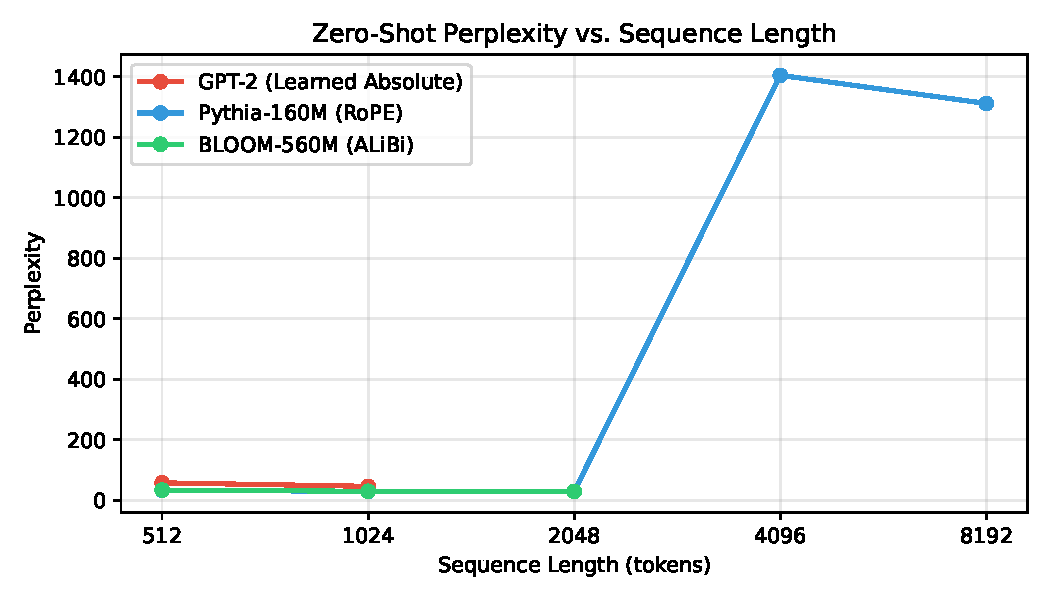
\includegraphics[width=\columnwidth]{figures/ppl_curves.pdf}
\caption{Zero-shot perplexity versus sequence length on a T4 GPU. RoPE and ALiBi track closely within the training window ($L \leq 2048$); RoPE degrades sharply past it. GPT-2 is limited to its 1024-token embedding ceiling.}
\label{fig:ppl}
\end{figure}

\begin{figure}[!t]
\centering
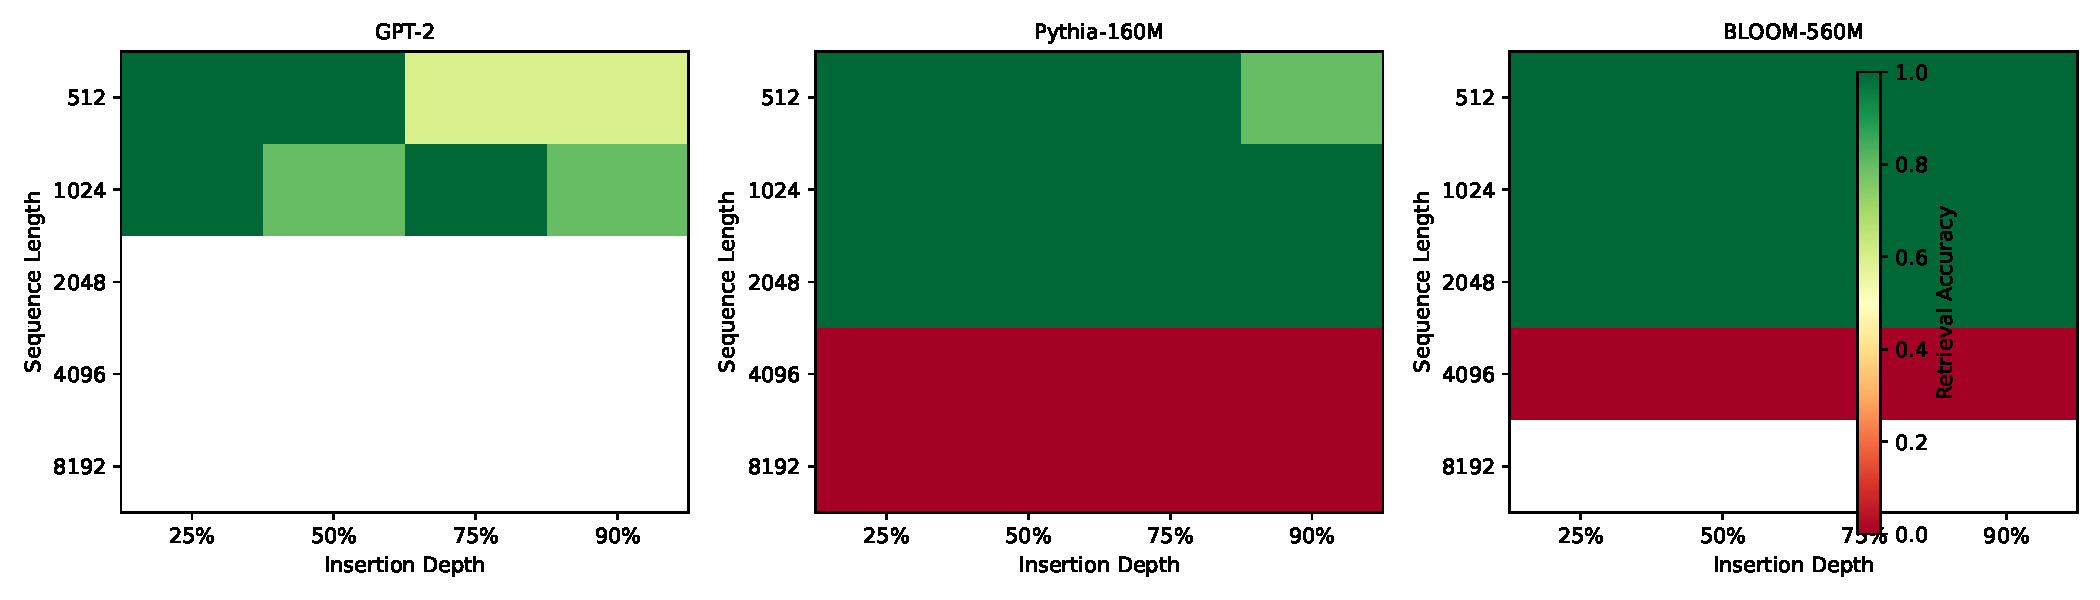
\includegraphics[width=\columnwidth]{figures/needle_heatmaps.pdf}
\caption{Needle retrieval accuracy heatmaps across insertion depths (25--90\%) and sequence lengths. All methods retrieve perfectly inside the training window; both RoPE and ALiBi collapse to 0\% beyond it.}
\label{fig:needle}
\end{figure}

\begin{figure}[!t]
\centering
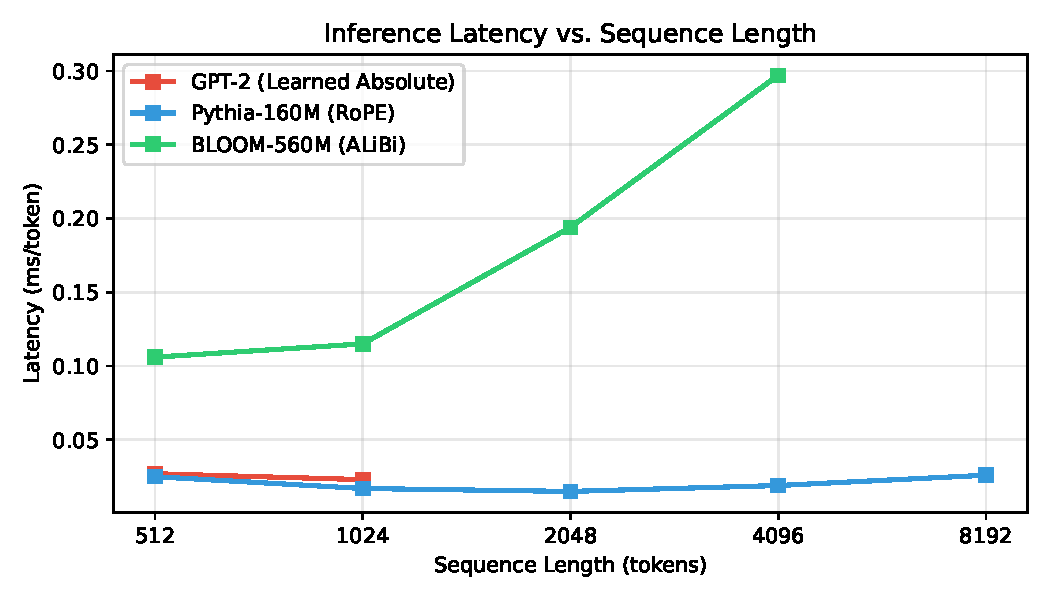
\includegraphics[width=\columnwidth]{figures/latency_curves.pdf}
\caption{Per-token inference latency versus sequence length on a T4 GPU.}
\label{fig:latency}
\end{figure}

\subsection{Limitations}

Four limitations bound the scope of these results. First, the three models differ in size (124M, 160M, 559M parameters) and vocabulary (50K--250K tokens), so cross-model perplexity and latency gaps may reflect capacity rather than the positional encoding alone; a controlled study training identical architectures from scratch would isolate the encoding effect. Second, BLOOM could not be evaluated at $L \geq 4096$ because its 250K-token output projection exceeds the 16\,GB T4 memory budget, truncating the ALiBi curve at the point where RoPE already shows degradation. Third, all measurements are single-run zero-shot evaluations; no confidence intervals or fine-tuned baselines (e.g., Position Interpolation, YaRN) are reported. Fourth, the synthetic needle task uses short, fixed phrases and may not reflect the retrieval demands of natural long-form documents.

\section{Conclusion}
\label{sec:conclusion}

This paper presented an empirical comparison of three positional encoding paradigms---Learned Absolute, RoPE, and ALiBi---evaluated under zero-shot conditions on a single GPU. Our experiments yield three key findings. First, within the training window, all three methods retrieve effectively (80--100\% needle accuracy) and both RoPE and ALiBi reach comparable perplexity (29.27--29.28 at $L{=}2048$), while Learned Absolute is capped at its 1024-token architectural limit. Second, neither RoPE nor ALiBi enables reliable zero-shot extrapolation: RoPE perplexity degrades $48\times$ at $L{=}4096$ and retrieval accuracy collapses to 0\%, while ALiBi retains perfect retrieval only through its training window and fails at $2\times$ its training length. Third, these findings align with the broader literature indicating that post-training scaling methods such as Position Interpolation and YaRN are required for meaningful length extrapolation, since the raw extrapolation capability of base models is limited regardless of the positional encoding mechanism.

Future research directions should focus on addressing the trade-offs of existing scaling techniques, particularly by investigating hybrid encodings that combine relative coordinate properties with implicit positional indicators. Additionally, further studies are needed to evaluate length generalization in non-causal attention models and to establish unified, downstream task-based benchmarks that look beyond simple perplexity evaluations.

\begin{thebibliography}{00}
\bibitem{vaswani2017} A. Vaswani et al., ``Attention is all you need,'' in \emph{Advances in Neural Information Processing Systems (NeurIPS)}, 2017, pp. 5998--6008.
\bibitem{touvron2023} H. Touvron et al., ``Llama: Open and efficient foundation language models,'' \emph{arXiv preprint arXiv:2302.13971}, 2023.
\bibitem{devlin2019} J. Devlin, M. W. Chang, K. Lee, and K. Toutanova, ``BERT: Pre-training of deep bidirectional transformers for language understanding,'' in \emph{Proceedings of the 2019 Conference of the North American Chapter of the Association for Computational Linguistics (NAACL-HLT)}, 2019, pp. 4171--4186.
\bibitem{radford2019} A. Radford, J. Wu, R. Child, D. Luan, D. Amodei, and I. Sutskever, ``Language models are unsupervised multitask learners,'' \emph{OpenAI blog}, vol. 1, no. 8, p. 9, 2019.
\bibitem{press2022} O. Press, N. A. Smith, and M. Lewis, ``Train short, test long: Attention with linear biases enables input length extrapolation,'' in \emph{International Conference on Learning Representations (ICLR)}, 2022.
\bibitem{raffel2020} C. Raffel et al., ``Exploring the limits of transfer learning with a unified text-to-text transformer,'' \emph{Journal of Machine Learning Research}, vol. 21, no. 140, pp. 1--67, 2020.
\bibitem{shaw2018} P. Shaw, J. Uszkoreit, and A. Vaswani, ``Self-attention with relative position representations,'' in \emph{Proceedings of the 2018 Conference of the North American Chapter of the Association for Computational Linguistics (NAACL-HLT)}, 2018, pp. 464--468.
\bibitem{dai2019} Z. Dai, Z. Yang, Y. Yang, J. Carbonell, Q. V. Le, and R. Salakhutdinov, ``Transformer-XL: Attentive language models beyond a fixed-length context,'' in \emph{Proceedings of the 57th Annual Meeting of the Association for Computational Linguistics (ACL)}, 2019, pp. 2978--2988.
\bibitem{su2024roformer} J. Su, Y. Lu, S. Pan, A. Murtadha, B. Wen, and Y. Liu, ``RoFormer: Enhanced Transformer with Rotary Position Embedding,'' \emph{Neurocomputing}, vol. 568, p. 127063, 2024.
\bibitem{chen2023} S. Chen et al., ``Extending context window of large language models via positional interpolation,'' \emph{arXiv preprint arXiv:2306.15595}, 2023.
\bibitem{liu2024scaling} X. Liu, H. Yan, S. Zhang, C. An, X. Qiu, and D. Lin, ``Scaling Laws of RoPE-based Extrapolation,'' in \emph{International Conference on Learning Representations (ICLR)}, 2024.
\bibitem{peng2023yarn} B. Peng, J. Quesnelle, H. Fan, and E. Shippole, ``YaRN: Efficient Context Window Extension of Large Language Models,'' \emph{arXiv preprint arXiv:2309.00071}, 2023.
\bibitem{sun2022lex} Y. Sun, L. Dong, B. Patra, S. Ma, S. Huang, A. Benhaim, V. Chaudhary, X. Song, and F. Wei, ``A Length-Extrapolatable Transformer,'' \emph{arXiv preprint arXiv:2212.10554}, 2022.
\bibitem{kazemnejad2023} A. Kazemnejad, I. Padhi, K. Natesan Ramamurthy, P. Das, and S. Reddy, ``The Impact of Positional Encoding on Length Generalization in Transformers,'' in \emph{Advances in Neural Information Processing Systems (NeurIPS)}, 2023.
\bibitem{ruoss2023} A. Ruoss, G. Del\'{e}tang, T. Genewein, J. Grau-Moya, R. Csord\'{a}s, M. Bennani, S. Legg, and J. Veness, ``Randomized Positional Encodings Boost Length Generalization of Transformers,'' in \emph{Proceedings of the 61st Annual Meeting of the Association for Computational Linguistics (Volume 2: Short Papers)}, 2023, pp. 1889--1903.
\bibitem{chi2022} T.-C. Chi, T.-H. Fan, P. Ramadge, and A. Rudnicky, ``KERPLE: Kernelized Relative Positional Embedding for Length Extrapolation,'' in \emph{Advances in Neural Information Processing Systems (NeurIPS)}, 2022.
\bibitem{zhao2024survey} L. Zhao, X. Feng, X. Feng, W. Zhong, D. Xu, Q. Yang, H. Liu, B. Qin, and T. Liu, ``Length Extrapolation of Transformers: A Survey from the Perspective of Positional Encoding,'' in \emph{Findings of the Association for Computational Linguistics: EMNLP 2024}, 2024, pp. 9959--9977.
\bibitem{veisi2025cable} A. Veisi, H. Amirzadeh, and A. Mansourian, ``Context-aware Biases for Length Extrapolation,'' \emph{arXiv preprint arXiv:2503.08067}, 2025.
\bibitem{shang2025longrope2} N. Shang, L. L. Zhang, S. Wang, G. Zhang, G. Lopez, F. Yang, W. Chen, and M. Yang, ``LongRoPE2: Near-Lossless LLM Context Window Scaling,'' \emph{arXiv preprint arXiv:2502.20082}, 2025.
\bibitem{he2024bipe} Z. He, G. Feng, S. Luo, K. Yang, D. He, J. Xu, Z. Zhang, H. Yang, and L. Wang, ``Two Stones Hit One Bird: Bilevel Positional Encoding for Better Length Extrapolation,'' in \emph{Proceedings of the 41st International Conference on Machine Learning (ICML)}, 2024.
\end{thebibliography}

\end{document}
